\documentclass[10pt]{article}
\usepackage{icmlko}

\icmlmeta{IP 파운데이션 월드모델}{4}{접근성과 유인}{라벨을 정리하자 다섯 축이 처음으로 상수를 이겼다}

\begin{document}

\twocolumn[
\icmlheader

\begin{abstract}
앞선 세 노트는 전부 진단이었다. 라벨 풀이 두 물리량을 섞고 있고(노트 1), 스코프와 시점이
어긋나 있으며(노트 2), 주최자 발표는 측정이 아니라 이산 어휘였다(노트 3). 이 노트는
그 진단을 실행에 옮긴다. 실제 계수만 남긴 75건의 풀에서 피처를 132개에서 줄여 가며
검정한 결과, \textbf{다섯 개 속성에서 처음으로 상수 중앙값을 유의하게 이겼다}
(차이 $-$0.0540, 95\% 신뢰구간 $-$0.103에서 $-$0.010). 132개 전부로는 이기지 못했고
(차이 $-$0.0315, 신뢰구간이 0을 포함), 셋으로 줄이면 다시 못 이겼다. 최적점은 다섯이다.
남은 다섯은 타깃 폭, 매장 노출도, 입장 허들, 미디어 투입, 굿즈 규모이며 --- 정리하면
\textbf{대상이 얼마나 넓은가, 닿기 얼마나 쉬운가, 닿으면 무엇을 얻는가}의 세 축이다.
제거했을 때 오히려 성능이 좋아진 두 속성은 IP 인지 폭과 콜라보 강도였다. \emph{IP가
얼마나 유명한지는 방문객 수를 설명하지 못한다.} 이 다섯 축은 팝업에 국한되지 않는
형태이며, IP 파운데이션 월드모델의 도메인 불변 골격 후보다.
\end{abstract}
]

\section{진단에서 실행으로}

이 연구의 목표는 IP가 대중과 만나는 모든 접점의 반응을 하나의 모델로 다루는 것이다.
첫 도메인인 팝업스토어에서 우리는 오랫동안 같은 벽에 부딪혔다 --- 어떤 모델도 상수
중앙값을 유의하게 이기지 못했다.

앞선 세 노트는 그 벽의 정체를 밝혔다. 라벨이 문제였다.

\begin{itemize}[leftmargin=1.1em,itemsep=0.15em]
\item 노트 1: 주최자 발표와 현장 계수가 2.75배 벌어져 한 컬럼에 섞여 있다.
\item 노트 2: 중간 집계에 전체 기간을 분모로 써서 21건의 일평균이 중앙 3.25배 과소평가됐다.
\item 노트 3: 주최자 발표 294건의 고유값은 86개뿐이고 상위 12개가 57\%를 차지한다.
      이산 어휘이며 정보가 소실됐다.
\end{itemize}

세 진단의 결론은 하나였다. \textbf{학습에 쓸 수 있는 것은 실제 계수 계열뿐이다.}
게이트 계수 49건과 체험 참여 계수 29건, 스코프 게이트를 통과하고 신뢰등급 A/B인
\textbf{75건}이 그 전부다.

이 노트는 그 75건 위에서 처음으로 모델을 다시 세운다.

\section{피처가 많을수록 나쁘다}

75건에 132개 피처는 명백히 과하다. Riley 등(2019)의 표본 크기 공식에 우리 조건을
대입하면 $p{=}132$, $R^2{=}0.15$일 때 필요 표본은 $n \approx 7{,}240$ --- 현재의 97배다.
$p{=}5$로 줄이면 $n \approx 274$로 3.7배까지 내려온다.

그래서 피처 집합을 단계적으로 줄이며 검정했다. 평가는 앞선 노트와 동일하게 IP 단위로
묶고 시간 순서를 강제하는 교차검증이며, 상수 중앙값 대비 페어드 부트스트랩 95\%
신뢰구간으로 판정한다.

\begin{figure}[t]\centering
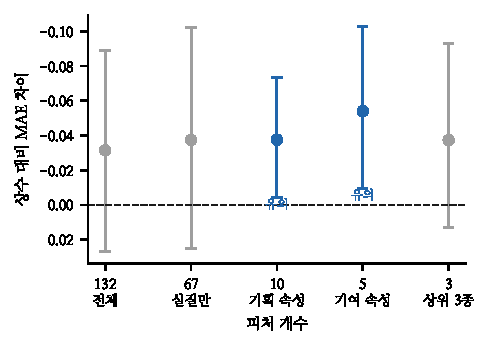
\includegraphics[width=\linewidth]{figs/feature_curve.pdf}
\caption{피처 개수와 성능. 점은 상수 대비 MAE 차이(아래가 좋음), 막대는 95\% 신뢰구간.
푸른색이 신뢰구간이 0을 넘지 않는 --- 즉 유의한 --- 지점이다.}
\label{fig:curve}
\end{figure}

\begin{table}[t]\centering\tsize
\caption{피처 집합별 결과. 계수 계열 $n{=}75$, 4폴드. 상수 MAE는 0.4427.}
\label{tab:sets}
\begin{tabular}{lrrl}
\toprule
피처 집합 & $p$ & MAE & 상수 대비 \\
\midrule
전체 & 132 & 0.4112 & $-0.0315$\ \ CI$[-0.089,+0.027]$ \\
실질만 & 67 & 0.4053 & $-0.0375$\ \ CI$[-0.102,+0.025]$ \\
기획 속성 & 10 & 0.4052 & $-0.0376$\ \ CI$[-0.074,-0.004]$ \\
\textbf{기여 속성} & \textbf{5} & \textbf{0.3888} & $\mathbf{-0.0540}$\ \ CI$[-0.103,-0.010]$ \\
상위 3종 & 3 & 0.4053 & $-0.0374$\ \ CI$[-0.093,+0.013]$ \\
\bottomrule
\end{tabular}
\end{table}

\claimx{피처를 132개에서 5개로 줄이자 처음으로 상수를 유의하게 이겼다
($\Delta=-0.0540$, CI$[-0.103,-0.010]$). 132개로는 이기지 못했고 3개로 줄이면 다시 못 이겼다.}
{다섯 개 집합은 열 개 안에서 leave-one-out 결과를 보고 고른 것이므로, 같은 데이터에서
고르고 같은 데이터에서 검정한 선택 편향이 있다. 새 표본에서 재현되는지 확인해야 한다.
$n{=}75$, 4폴드에서 신뢰구간 상단이 $-0.010$으로 0에 가깝다는 점도 감안해야 한다.}

\section{어느 속성이 기여하는가}

열 개의 기획 속성은 모두 0--4 척도의 순서형이다. 원문 문서를 읽어 태깅한 것으로,
체험 요소의 밀도, 굿즈 규모, 포토존 수, 콜라보 강도, IP의 대중 인지 폭, 타깃 폭,
입장 허들, 미디어 투입, 시즌 적합성, 매장 내 노출도를 잰다.

각 속성을 하나씩 빼고 나머지 아홉으로 학습해, 뺐을 때 오차가 얼마나 늘어나는지를 재었다.

\begin{figure}[t]\centering
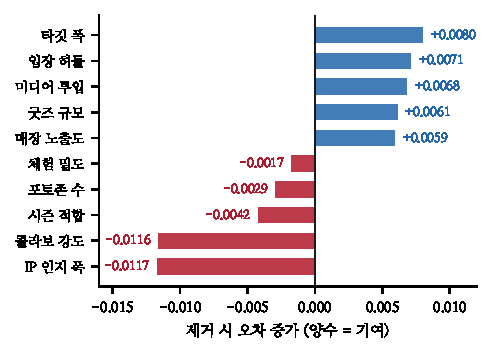
\includegraphics[width=\linewidth]{figs/attr_contrib.pdf}
\caption{속성별 기여. 양수(푸른색)는 제거 시 오차가 늘어나는 --- 즉 기여하는 --- 속성이고,
음수(붉은색)는 제거 시 오히려 좋아지는 속성이다.}
\label{fig:contrib}
\end{figure}

다섯이 기여하고, 셋은 중립이며, \textbf{둘은 해롭다}.

\begin{table}[t]\centering\tsize
\caption{기여 속성과 타깃의 스피어만 상관($n{=}75$).}
\label{tab:corr}
\begin{tabular}{lrr}
\toprule
속성 & $\rho$ & $p$ \\
\midrule
타깃 폭 & $+0.362$ & 0.001 \\
매장 노출도 & $+0.358$ & 0.002 \\
미디어 투입 & $+0.273$ & 0.018 \\
굿즈 규모 & $+0.250$ & 0.031 \\
입장 허들 & $-0.236$ & 0.041 \\
\midrule
콜라보 강도 & $+0.153$ & 0.191 \\
IP 인지 폭 & --- & --- \\
\bottomrule
\end{tabular}
\end{table}

\claimx{IP 인지 폭과 콜라보 강도는 제거하면 성능이 좋아진다
(각각 $-0.0117$, $-0.0116$). \emph{IP가 얼마나 유명한지는 방문객 수를 설명하지 못한다.}}
{두 속성이 다른 다섯과 상관돼 있어 다중공선성으로 계수가 불안정해진 결과일 수 있다.
또한 우리 태깅에서 IP 인지 폭은 ``대중 인지''를 재는데, 방문객을 결정하는 것은 인지가
아니라 \emph{동원력}일 수 있다. 두 개념을 분리해 다시 태깅하면 결과가 바뀔 수 있다.}

이 결과는 직관에 반하지만 개념적으로는 설명된다. 대중 인지도가 높은 IP --- 예컨대
전 국민이 이름을 아는 연예인 --- 라도 그 인지가 오프라인 방문으로 이어지지는 않는다.
23년간 단독 공연을 한 번도 하지 않은 톱스타의 팝업과, 인지도는 낮지만 코어 팬덤이
단단한 IP의 팝업 중 어느 쪽에 사람이 더 오는가는 인지도로 답할 수 없다.

\section{남은 다섯의 구조}

기여하는 다섯을 늘어놓으면 세 갈래로 묶인다.

\begin{figure*}[t]\centering
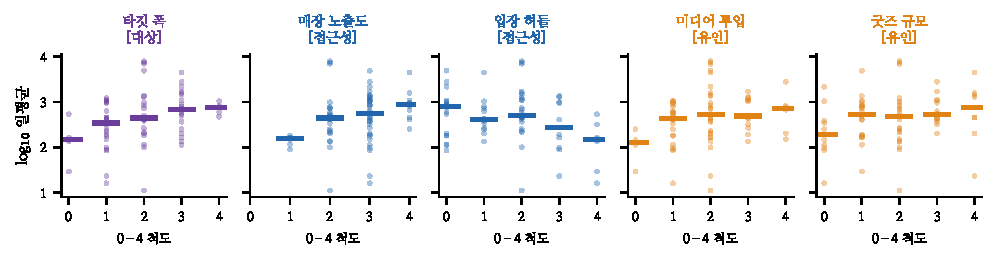
\includegraphics[width=\linewidth]{figs/five_axes.pdf}
\caption{다섯 속성과 타깃의 관계. 각 패널은 0--4 척도별 분포이며 가로 막대는 중앙값이다.
색은 세 갈래를 구분한다 --- 대상(보라), 접근성(파랑), 유인(주황).}
\label{fig:axes}
\end{figure*}

\paragraph{대상 --- 누구를 향하는가}
타깃 폭($\rho=+0.362$)이 가장 강한 단일 신호다. 코어 팬덤만 겨냥한 팝업과 전 연령을
겨냥한 팝업 사이에 방문객이 갈린다.

\paragraph{접근성 --- 닿기 얼마나 쉬운가}
매장 노출도($+0.358$)와 입장 허들($-0.236$)이 반대 부호로 짝을 이룬다.
1층 정면에 있으면 지나가다 들어오고, 유료 사전예약이면 작정하고 와야 한다.

\paragraph{유인 --- 닿으면 무엇을 얻는가}
미디어 투입($+0.273$)과 굿즈 규모($+0.250$)다. 알려야 오고, 살 것이 있어야 온다.

\claimx{남은 다섯은 ``대상 $\times$ 접근성 $\times$ 유인'' 구조를 이룬다.
IP의 유명세가 아니라, 그 IP를 향한 사람이 얼마나 쉽게 닿고 닿으면 무엇을 얻는가다.}
{세 갈래 분류는 사후 해석이다. 다섯 속성이 실제로 세 잠재 요인으로 묶이는지는 요인분석
등으로 확인해야 하며, $n{=}75$에서는 그 검정 자체의 검정력이 부족하다.}

\section{왜 이것이 파운데이션 모델의 골격인가}

이 다섯 축은 팝업스토어의 언어로 쓰였지만, 팝업에만 있는 것이 아니다.

아이돌 데뷔를 생각해 보자. \emph{대상 폭}은 코어 팬덤을 겨냥한 앨범인지 대중을 겨냥한
곡인지다. \emph{접근성}은 음원 스트리밍(허들 0)과 콘서트 티켓(허들 4)의 차이이며,
음악방송 출연은 매장 노출도에 해당한다. \emph{유인}은 미디어 투입과 앨범 구성
(포토카드·특전)이다.

광고 모델 기용도 같은 구조로 읽힌다. 게임 출시도 마찬가지다.
반면 이번에 탈락한 ``IP 인지 폭''은 도메인마다 의미가 달라지는 축이었다.

\claimx{다섯 축은 도메인 불변 형태로 기술된다. IP 파운데이션 월드모델의 공유 표현
후보로서, 도메인별로 다른 것은 축의 \emph{값}이지 축 자체가 아니다.}
{이는 아직 가설이다. 아이돌 도메인에서 같은 다섯 축을 태깅해 전이가 실제로 일어나는지
검정하지 않았다. 앞선 문헌 검토에서 소표본 도메인 간 전이는 부정적 결과가 지배적이었으므로
(Standley 등 2020, Ben-David 등 2010), 기대치를 낮게 잡아야 한다.}

\section{한계}

정직하게 적어야 할 것이 여럿이다.

\textbf{선택 편향.} 다섯 속성은 열 개 안에서 leave-one-out을 보고 골랐고, 같은 데이터로
검정했다. 이 절차는 낙관적이다. 엄밀하게는 속성 선택을 폴드 안에서 수행하는 중첩
교차검증이 필요하다.

\textbf{경계에 있는 유의성.} $\Delta=-0.0540$의 신뢰구간 상단이 $-0.010$이다.
0에서 멀지 않다. 표본이 몇 건 바뀌면 판정이 뒤집힐 수 있다 --- 실제로 앞선 세션에서
라벨 5건이 바뀌자 모델 순위가 뒤집힌 적이 있다.

\textbf{여전히 작은 개선.} 오차 배율로 보면 2.77배에서 2.45배다. 실무에서 ``2.5배 안에
들어온다''는 것은 500명 예측에 200--1{,}250명 구간을 뜻한다. 쓸 만한 예측이라 하기 어렵다.

\textbf{태깅의 주관성.} 다섯 속성은 원문을 읽고 0--4로 매긴 값이다. 같은 문서를 다른
평가자가 매기면 얼마나 일치하는지 재지 않았다.

\section{다음 단계}

\paragraph{즉시}
속성 선택을 폴드 안으로 넣은 중첩 교차검증으로 다섯 축의 유의성을 재확인한다.
그리고 태깅 재현성을 잰다 --- 같은 문서를 두 번 태깅해 일치도를 본다.

\paragraph{표본}
Riley 기준으로 $p{=}5$에 필요한 표본은 $n \approx 274$다. 현재 75건에서 3.7배가
필요하다. 노트 3에서 확인했듯 발표 수치는 쓸 수 없으므로, 계수 라벨을 새로 확보하는
경로 --- 웨이팅 시스템 로그, 유통사 층별 집계 --- 를 열어야 한다.

\paragraph{도메인 확장}
아이돌 도메인의 레코드에 같은 다섯 축을 태깅하고, 전이가 일어나는지 검정한다.
이것이 파운데이션 모델 가설의 첫 시험이다.

\vspace{0.7em}
\hrule
\vspace{0.4em}
{\footnotesize\color{black!60}
평가 코드는 \texttt{state/evaluate.py}, 그림 생성은 \texttt{paper/figs.py}이며 모두
저장소 데이터에서 직접 계산한다. 라벨이 갱신되면 모든 수치가 함께 바뀐다.}

\end{document}
